% Presentación oral del TP3, basada en el formato Beamer final del TP2.
\documentclass[aspectratio=169,11pt]{beamer}
\usetheme{Warsaw}
\useoutertheme{miniframes}
\setbeamertemplate{navigation symbols}{}
\setbeamertemplate{footline}[frame number]

\usepackage[spanish,es-noquoting]{babel}
\usepackage{amsmath,amssymb,bm}
\usepackage{graphicx}
\usepackage{booktabs}
\usepackage{xcolor}
\usepackage{tikz}
\usetikzlibrary{positioning}

\definecolor{itbablue}{RGB}{0,91,145}
\definecolor{accent}{RGB}{211,92,32}
\definecolor{softblue}{RGB}{232,243,249}
\setbeamercolor{structure}{fg=itbablue}
\setbeamercolor{alerted text}{fg=accent}
\setbeamercolor{block title}{fg=white,bg=itbablue}
\setbeamercolor{block body}{bg=softblue}
\setbeamerfont{frametitle}{size=\large}
\setbeamerfont{title}{size=\LARGE}

\setbeamertemplate{section page}{%
  \begin{centering}
    \vfill
    {\usebeamercolor[fg]{structure}\usebeamerfont{title}\insertsectionhead\par}
    \vfill
  \end{centering}
}

\newcommand{\slot}[3]{%
  \fbox{\parbox[c][#2][c]{\dimexpr#1-2\fboxsep-2\fboxrule\relax}{\centering\footnotesize\color{gray}#3}}}
\newcommand{\pend}[1]{{\color{accent}\textbf{[#1]}}}
\newcommand{\parametros}[1]{{\small #1}}
\newcommand{\videolink}[1]{{\tiny\color{accent}\texttt{#1}}}

\title[Billar-Metegol]{Simulación dirigida por eventos de un Billar-Metegol}
\subtitle{Búsqueda de obstáculos para minimizar el tiempo al 90\,\% de goles}
\author[Grupo 07]{Grupo 07 - Comisión S\\Eugenio Migliaro, Francisco Costa y Franco Branda}
\institute{72.25 Simulación de Sistemas - ITBA}
\date{28 de septiembre de 2026}

\begin{document}

% 1
\begin{frame}
  \titlepage
\end{frame}

% 2
\section{Introducción}
\begin{frame}
  \sectionpage
\end{frame}

% 3
\begin{frame}{Sistema real}
  \begin{columns}[c,onlytextwidth]
    \begin{column}{0.56\textwidth}
      \centering
      \begin{tikzpicture}[x=5.4cm,y=5.4cm]
        \draw[very thick] (0,0) rectangle (1.2,0.68);
        \draw[line width=3pt,itbablue] (0,0.24) -- (0,0.44);
        \draw[line width=3pt,itbablue] (1.2,0.24) -- (1.2,0.44);
        \fill[accent] (0.60,0.34) circle (0.075);
        \fill[itbablue] (0.24,0.16) circle (0.023);
        \fill[itbablue] (0.87,0.51) circle (0.023);
        \fill[red!75!black] (1.04,0.27) circle (0.023);
        \draw[->,thick] (0.24,0.16) -- (0.34,0.22);
        \draw[->,thick] (0.87,0.51) -- (0.77,0.45);
        \node[rotate=90,anchor=south] at (-0.04,0.34) {arco};
        \node[rotate=90,anchor=north] at (1.24,0.34) {arco};
      \end{tikzpicture}
    \end{column}
    \begin{column}{0.40\textwidth}
      \begin{itemize}
        \item Partículas en movimiento rectilíneo entre colisiones.
        \item Choques elásticos con paredes, partículas y obstáculos.
        \item El primer contacto con un arco cambia su estado.
      \end{itemize}
      \begin{block}{Objetivo}
        Minimizar $\langle t_{90}\rangle$ mediante la configuración de obstáculos.
      \end{block}
    \end{column}
  \end{columns}
\end{frame}

% 4
\begin{frame}{Fundamentos}
  \begin{columns}[T,onlytextwidth]
    \begin{column}{0.47\textwidth}
      \begin{block}{Movimiento libre}
        \[
          \bm{x}_i(t+\tau)=\bm{x}_i(t)+\bm{v}_i(t)\,\tau
        \]
        Cada trayectoria se propaga hasta el próximo evento.
      \end{block}
    \end{column}
    \begin{column}{0.49\textwidth}
      \begin{block}{Choque elástico}
        \[
          \sum_i m_i\bm{v}_i^{\,-}=\sum_i m_i\bm{v}_i^{\,+},
          \qquad E_c^{-}=E_c^{+}
        \]
        Las paredes y los obstáculos producen reflexión especular.
      \end{block}
    \end{column}
  \end{columns}
  \vfill
  \centering\small El reloj avanza de colisión en colisión, con un paso temporal variable.
\end{frame}

% 5
\begin{frame}{Fundamentos}
  \begin{columns}[c,onlytextwidth]
    \begin{column}{0.58\textwidth}
      \begin{block}{Próximo evento}
        Para cada candidato se resuelve analíticamente su tiempo de choque
        $\tau_e\geq 0$ y se elige
        \[
          e^*=\operatorname*{arg\,min}_e\{t+\tau_e\}.
        \]
      \end{block}
      \begin{block}{Estado discreto}
        Una partícula fresca pasa a usada al tocar por primera vez un arco.
        Luego continúa colisionando sin volver a sumar un gol.
      \end{block}
    \end{column}
    \begin{column}{0.38\textwidth}
      \centering
      \begin{tikzpicture}[node distance=1.0cm,>=latex]
        \node[draw,rounded corners,fill=softblue,minimum width=2.8cm] (p) {predecir};
        \node[draw,rounded corners,fill=softblue,below of=p,minimum width=2.8cm] (a) {avanzar};
        \node[draw,rounded corners,fill=softblue,below of=a,minimum width=2.8cm] (r) {resolver};
        \draw[->,thick] (p) -- (a);
        \draw[->,thick] (a) -- (r);
        \draw[->,thick] (r.east) -- ++(0.55,0) |- (p.east);
      \end{tikzpicture}
    \end{column}
  \end{columns}
\end{frame}

% 6
\section{Implementación}
\begin{frame}
  \sectionpage
\end{frame}

% 7
\begin{frame}{Arquitectura del motor}
  \centering
  \begin{tikzpicture}[node distance=0.36cm, every node/.style={font=\small}]
    \node[draw,fill=softblue,minimum width=3.4cm,minimum height=0.58cm] (cli) {CLI y configuración};
    \node[draw,fill=softblue,below=of cli,minimum width=3.4cm,minimum height=0.58cm] (gen) {Generación del sistema};
    \node[draw,fill=softblue,below=of gen,minimum width=3.4cm,minimum height=0.58cm] (sim) {Motor dirigido por eventos};
    \node[draw,fill=softblue,below left=0.48cm and 0.25cm of sim,minimum width=3.2cm,minimum height=0.58cm] (col) {Predicción y colisiones};
    \node[draw,fill=softblue,below right=0.48cm and 0.25cm of sim,minimum width=3.2cm,minimum height=0.58cm] (geo) {Geometría y validación};
    \node[draw,fill=softblue,below=1.48cm of sim,minimum width=3.4cm,minimum height=0.58cm] (io) {Trayectoria de estados};
    \draw[->,thick] (cli) -- (gen);
    \draw[->,thick] (gen) -- (sim);
    \draw[->,thick] (sim) -- (col);
    \draw[->,thick] (sim) -- (geo);
    \draw[->,thick] (sim) -- (io);
  \end{tikzpicture}

  \vspace{0.15em}
  \begin{block}{Separación exigida}
    El motor genera tiempo, posiciones, velocidades y color. El posprocesamiento calcula $F_u$, $t_{90}$, DCM y $D$.
  \end{block}
\end{frame}

% 8
\begin{frame}{Estructuras principales}
  \begin{columns}[T,onlytextwidth]
    \begin{column}{0.48\textwidth}
      \begin{block}{System}
        \begin{itemize}
          \item \texttt{Table}: $L$, $W$ y $d$.
          \item \texttt{Particle}: $\bm{x}$, $\bm{v}$, estado y contador.
          \item \texttt{Obstacle}: centro y radio.
        \end{itemize}
      \end{block}
    \end{column}
    \begin{column}{0.48\textwidth}
      \begin{block}{Event}
        \begin{itemize}
          \item Instante absoluto y tipo de choque.
          \item Participantes del evento.
          \item Contadores al momento de agendar.
        \end{itemize}
      \end{block}
    \end{column}
  \end{columns}
  \vfill
  \centering
  \begin{tikzpicture}[every node/.style={font=\small},>=latex]
    \node[draw,fill=softblue,minimum width=2.4cm] (s) {System};
    \node[draw,fill=softblue,right=1.7cm of s,minimum width=2.4cm] (q) {EventQueue};
    \node[draw,fill=softblue,right=1.7cm of q,minimum width=2.4cm] (e) {Event};
    \draw[->,thick] (s) -- node[above]{agenda} (q);
    \draw[->,thick] (q) -- node[above]{extrae} (e);
  \end{tikzpicture}
\end{frame}

% 9
\begin{frame}{Algoritmo de simulación}
  \begin{columns}[T,onlytextwidth]
    \begin{column}{0.67\textwidth}
      \begin{beamercolorbox}[sep=0.6em,rounded=true]{block body}
        {\small\ttfamily
        estado $\leftarrow$ generar(configuración, semilla)\\[0.25em]
        cola $\leftarrow$ agendar todos los choques\\
        \textbf{mientras} cola no esté vacía:\\
        \quad evento $\leftarrow$ extraer mínimo\\
        \quad \textbf{si} evento está invalidado: continuar\\
        \quad \textbf{si} evento.t $>$ tmax: terminar\\
        \quad avanzar todas las partículas hasta evento.t\\
        \quad resolver(evento)\\
        \quad escribir estado si corresponde\\
        \quad reagendar participantes
        }
      \end{beamercolorbox}
    \end{column}
    \begin{column}{0.29\textwidth}
      \begin{block}{Invalidación perezosa}
        Un evento se invalida si cambió el contador de choques de algún participante.
      \end{block}
      \begin{block}{Costo}
        Cola: $O(N\log E)$ por evento; predomina el costo de reagendar participantes.
      \end{block}
    \end{column}
  \end{columns}
\end{frame}

% 10
\section{Simulaciones}
\begin{frame}
  \sectionpage
\end{frame}

% 11
\begin{frame}{Sistema particular}
  \begin{columns}[c,onlytextwidth]
    \begin{column}{0.55\textwidth}
      \centering
      \begin{tikzpicture}[x=5.35cm,y=5.35cm]
        \draw[very thick] (0,0) rectangle (1.2,0.68);
        \draw[line width=4pt,itbablue] (0,0.24) -- (0,0.44);
        \draw[line width=4pt,itbablue] (1.2,0.24) -- (1.2,0.44);
        \fill[accent] (0.62,0.34) circle (0.080);
        \draw[<->] (0,-0.07) -- node[below] {$L=1{,}20\ \mathrm{m}$} (1.2,-0.07);
        \draw[<->] (-0.07,0) -- node[rotate=90,above] {$W=0{,}68\ \mathrm{m}$} (-0.07,0.68);
        \draw[<->] (0.62,0.34) -- node[above] {$R_k$} (0.70,0.34);
        \draw[<->] (1.16,0.24) -- node[left] {$d$} (1.16,0.44);
        \fill[itbablue] (0.25,0.18) circle (0.0175);
        \draw[->,thick] (0.25,0.18) -- node[below] {$\bm{v}_i$} (0.38,0.23);
        \draw[<->] (0.25,0.18) -- node[left] {$r$} (0.25,0.1975);
      \end{tikzpicture}
    \end{column}
    \begin{column}{0.41\textwidth}
      {\scriptsize
      \begin{tabular}{@{}ll@{}}
        \toprule
        Partículas & $N=100$ \\
        Radio & $r=1{,}75\,10^{-2}\ \mathrm{m}$ \\
        Masa & $m=2{,}5\,10^{-2}\ \mathrm{kg}$ \\
        Rapidez inicial & $v_0=1\ \mathrm{m\,s^{-1}}$ \\
        Colisiones & elásticas \\
        \bottomrule
      \end{tabular}}
      \vspace{0.5em}
      \begin{block}{Configuración}
        $K>0$ discos fijos, $R_k\geq r$, contenidos y sin solaparse.
      \end{block}
    \end{column}
  \end{columns}
\end{frame}

% 12
\begin{frame}{Protocolo experimental}
  \begin{columns}[T,onlytextwidth]
    \begin{column}{0.47\textwidth}
      \begin{block}{Parámetros físicos}
        $N$, $L$, $W$, $d$, $r$, $m$, $v_0$ y $(x_k,y_k,R_k)$.
      \end{block}
      \begin{block}{1.1 Rendimiento}
        Mesa vacía, $t_f=30\ \mathrm{s}$, al menos 10 realizaciones por $N$.
      \end{block}
    \end{column}
    \begin{column}{0.49\textwidth}
      \begin{block}{1.2 Configuraciones}
        Mesa vacía y familias de obstáculos, con al menos 5 realizaciones por punto.
      \end{block}
      \begin{block}{Datos de ejecución}
        $t_{\max}$, semilla, cadencia de guardado y cantidad de realizaciones no son parámetros físicos.
      \end{block}
    \end{column}
  \end{columns}
\end{frame}

% 13
\begin{frame}{Goles y tiempo característico}
  \begin{columns}[T,onlytextwidth]
    \begin{column}{0.47\textwidth}
      \textbf{Fracción de partículas usadas}
      \[
        F_u^{(s)}(t)=\frac{N_g^{(s)}(t)}{N}.
      \]
      \textbf{Tiempo por realización}
      \[
        t_{90}^{(s)}=\min\{t:F_u^{(s)}(t)\geq0{,}9\}.
      \]
    \end{column}
    \begin{column}{0.49\textwidth}
      \begin{block}{Promedio entre realizaciones}
        \[
          \langle t_{90}\rangle=\frac{1}{n_r}\sum_{s=1}^{n_r}t_{90}^{(s)}
        \]
        \[
          \sigma_{t_{90}}=\sqrt{\frac{1}{n_r-1}\sum_{s=1}^{n_r}
          \left(t_{90}^{(s)}-\langle t_{90}\rangle\right)^2}.
        \]
      \end{block}
      \small Las corridas que no llegan al 90\,\% antes de $t_{\max}$ se informan, no se descartan.
    \end{column}
  \end{columns}
\end{frame}

% 14
\begin{frame}{Difusión}
  \begin{columns}[T,onlytextwidth]
    \begin{column}{0.51\textwidth}
      \textbf{Desplazamiento cuadrático medio}
      \[
        \mathrm{DCM}^{(s)}(t)=\frac{1}{N}\sum_{i=1}^{N}
        \left\lVert\bm{x}_i^{(s)}(t)-\bm{x}_i^{(s)}(0)\right\rVert^2.
      \]
      En la ventana difusiva:
      \[
        \mathrm{DCM}(t)=4Dt.
      \]
    \end{column}
    \begin{column}{0.45\textwidth}
      \begin{block}{Ajuste por realización}
        \[
          E(c)=\sum_j\left[\mathrm{DCM}(t_j)-c\,t_j\right]^2
        \]
        \[
          D=\frac{c_{\min}}{4}.
        \]
      \end{block}
      \begin{block}{Reporte}
        Se calcula $D^{(s)}$ para cada semilla y luego $\langle D\rangle\pm\sigma_D$.
      \end{block}
    \end{column}
  \end{columns}
\end{frame}

% 15
\section{Resultados}
\begin{frame}
  \sectionpage
\end{frame}

% 16
\begin{frame}{Dinámica del sistema}
  \begin{columns}[T,onlytextwidth]
    \begin{column}{0.47\textwidth}
      \centering
      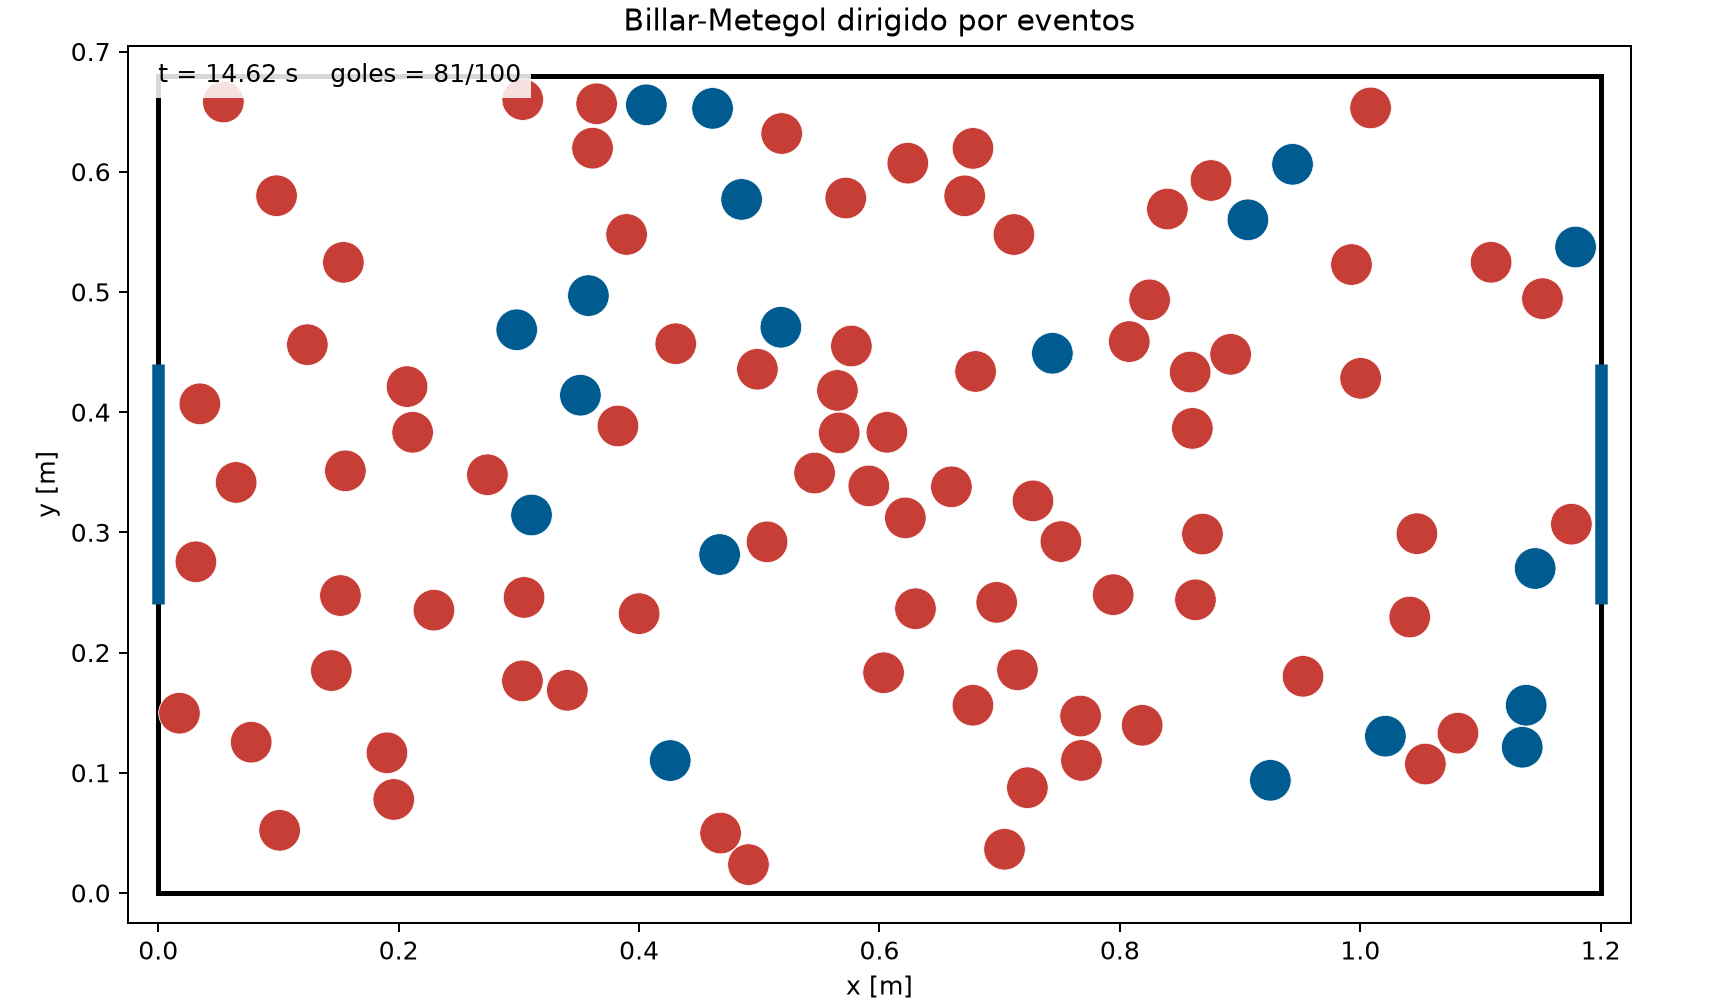
\includegraphics[width=\textwidth,height=3.7cm,keepaspectratio]{figuras/anim-vacia.png}\\[3pt]
      \videolink{URL YouTube/Vimeo pendiente de publicación}
    \end{column}
    \begin{column}{0.47\textwidth}
      \centering
      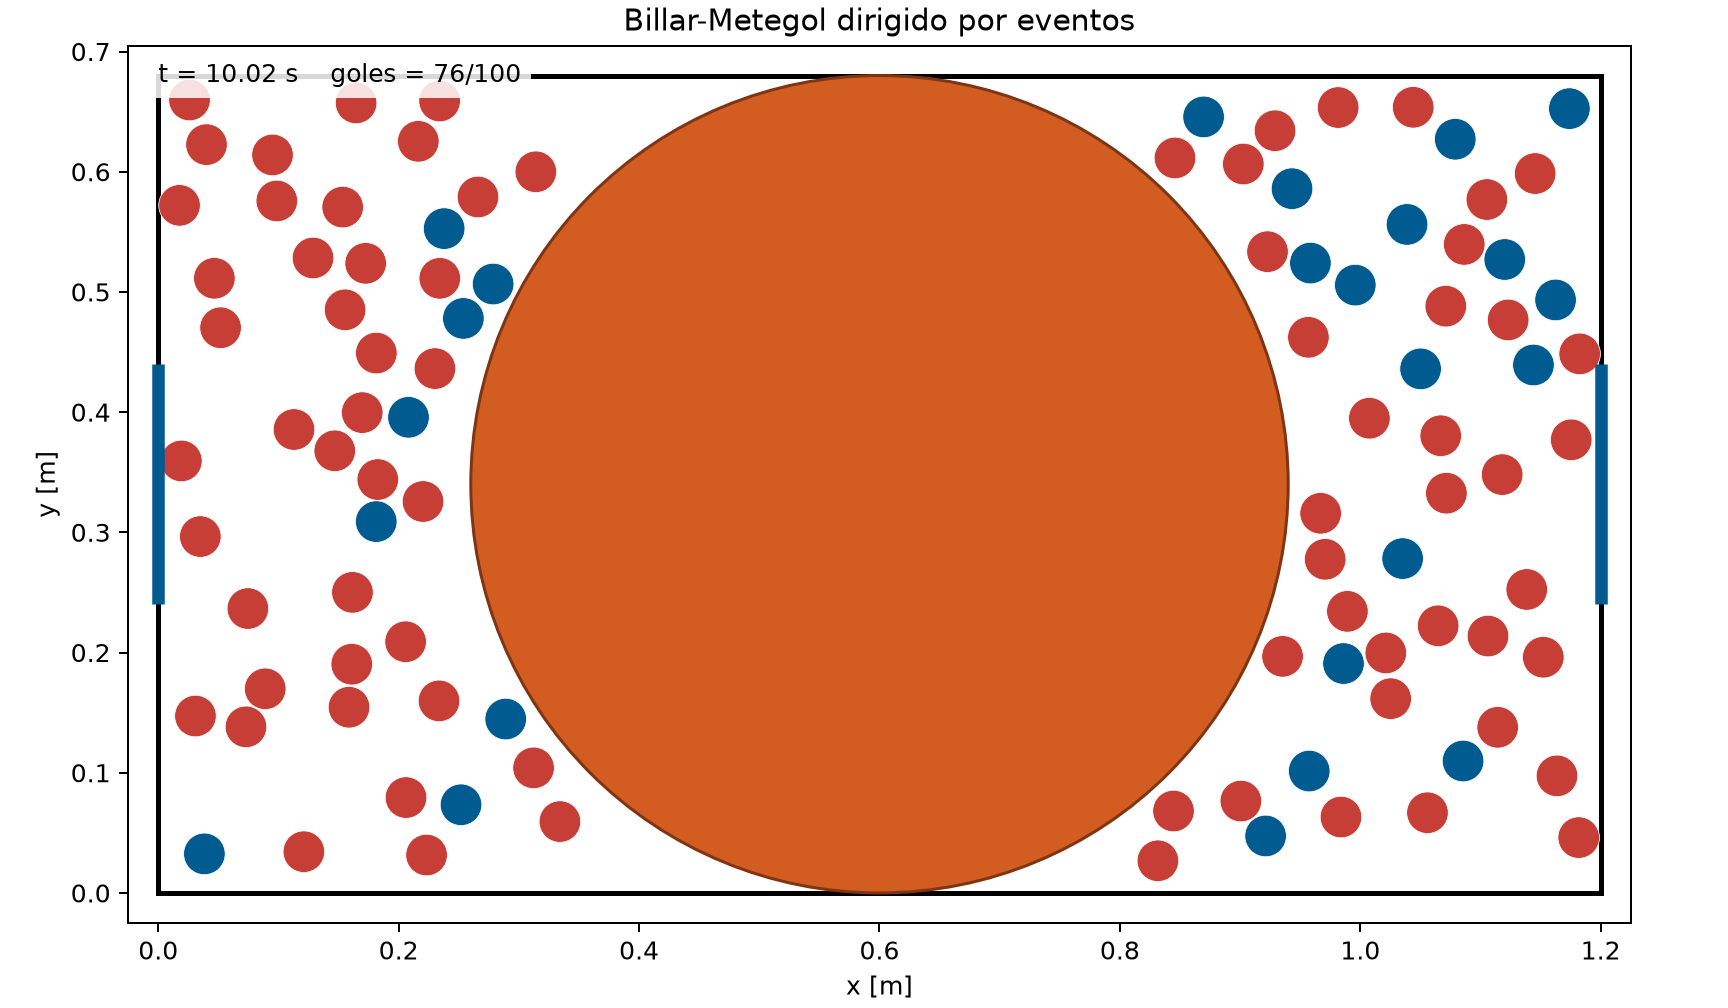
\includegraphics[width=\textwidth,height=3.7cm,keepaspectratio]{figuras/anim-mejor.png}\\[3pt]
      \videolink{URL YouTube/Vimeo pendiente de publicación}
    \end{column}
  \end{columns}
  \vspace{0.4em}
  \centering\parametros{$N=100$, $v_0=1\ \mathrm{m\,s^{-1}}$, $r=1{,}75\,10^{-2}\ \mathrm{m}$; semillas 2006 y 2010.}
\end{frame}

% 17
\begin{frame}{Tiempo de ejecución en función de $N$}
  \centering
  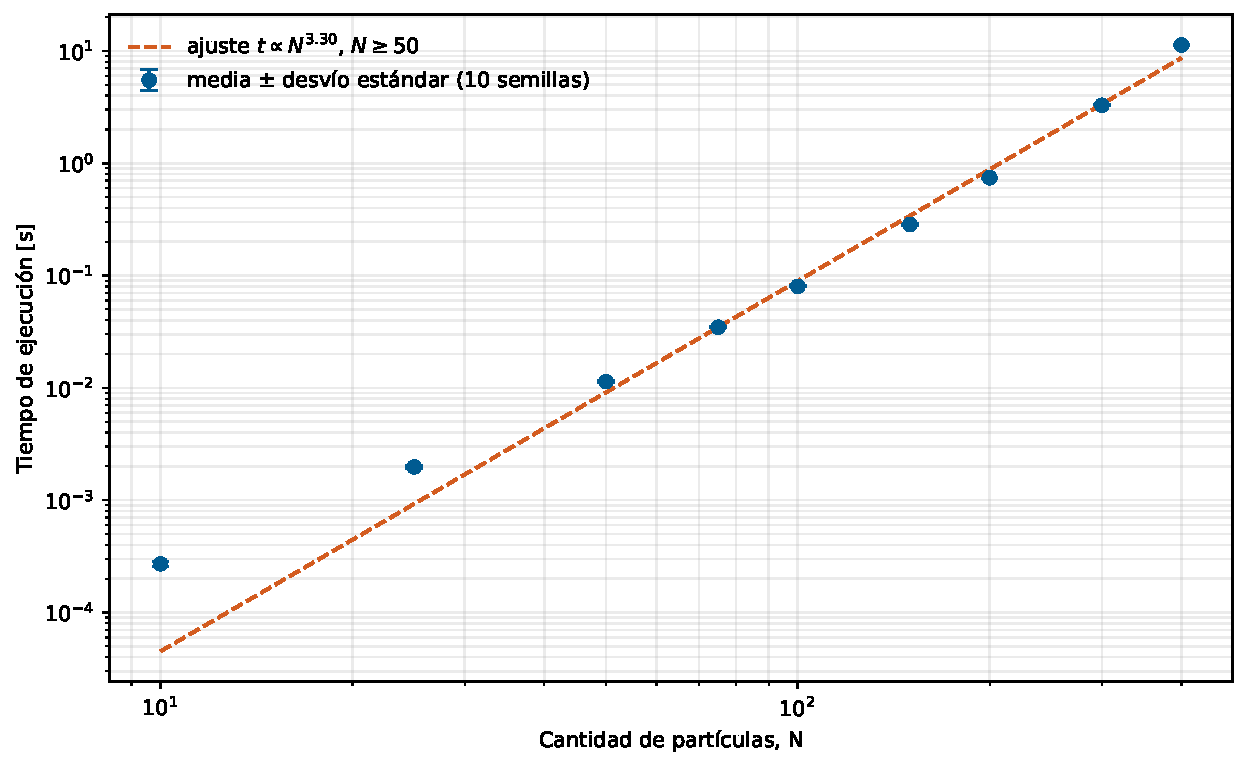
\includegraphics[width=\textwidth,height=5.25cm,keepaspectratio]{figuras/runtime-vs-N.pdf}
  \vspace{0.2em}
  \par\parametros{Mesa vacía; $t_f=30\ \mathrm{s}$; 10 realizaciones por $N$; motor con cola de prioridad.\\
  En $50\leq N\leq400$, $t\propto N^{3{,}30}$; para $N=400$, $t=11{,}27\pm0{,}04\ \mathrm{s}$.}
\end{frame}

% 18
\begin{frame}{Evolución de la fracción usada}
  \centering
  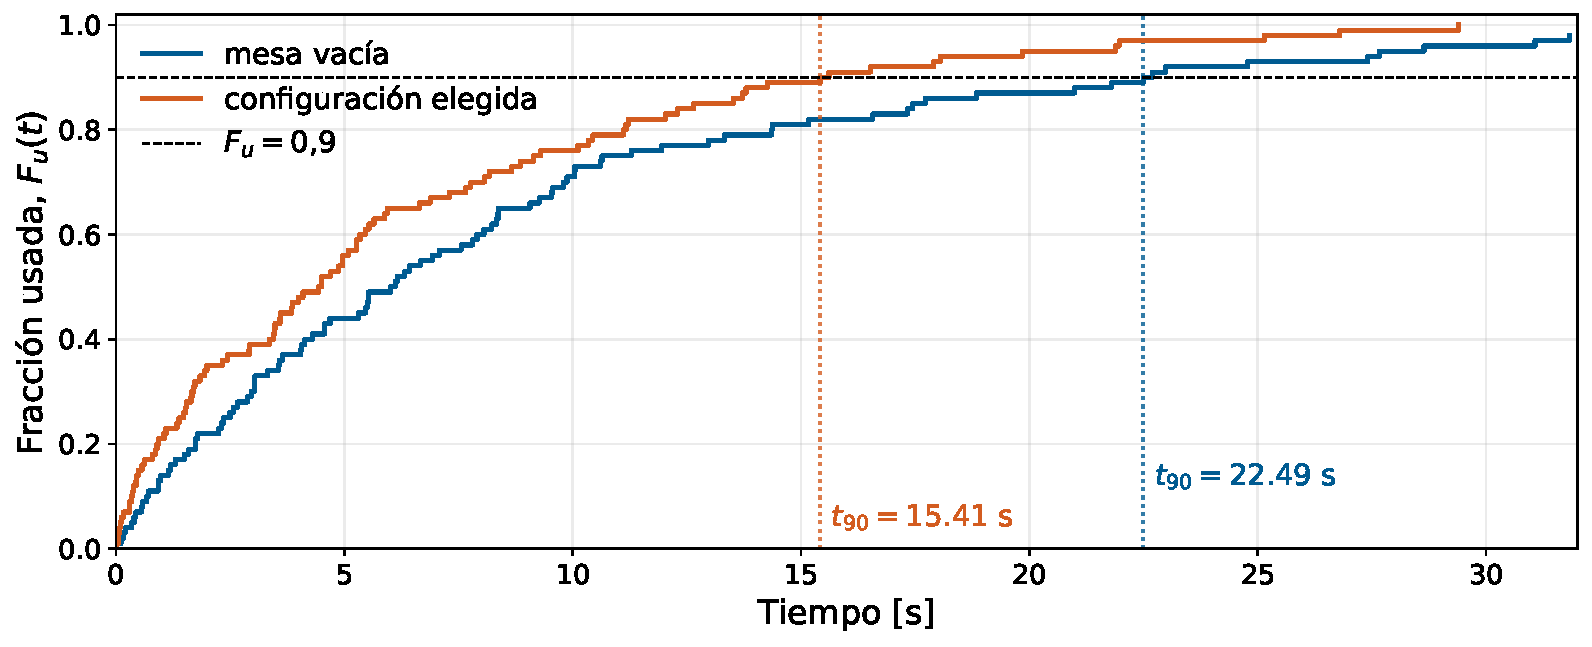
\includegraphics[width=\textwidth,height=5.25cm,keepaspectratio]{figuras/Fu-vs-tiempo.pdf}
  \vspace{0.2em}
  \par\parametros{$N=100$; mesa vacía: semilla 2006; configuración elegida: semilla 2010.\\
  Se calcula $t_{90}$ por realización antes de promediar.}
\end{frame}

% 19
\begin{frame}{Exploración de configuraciones}
  \centering
  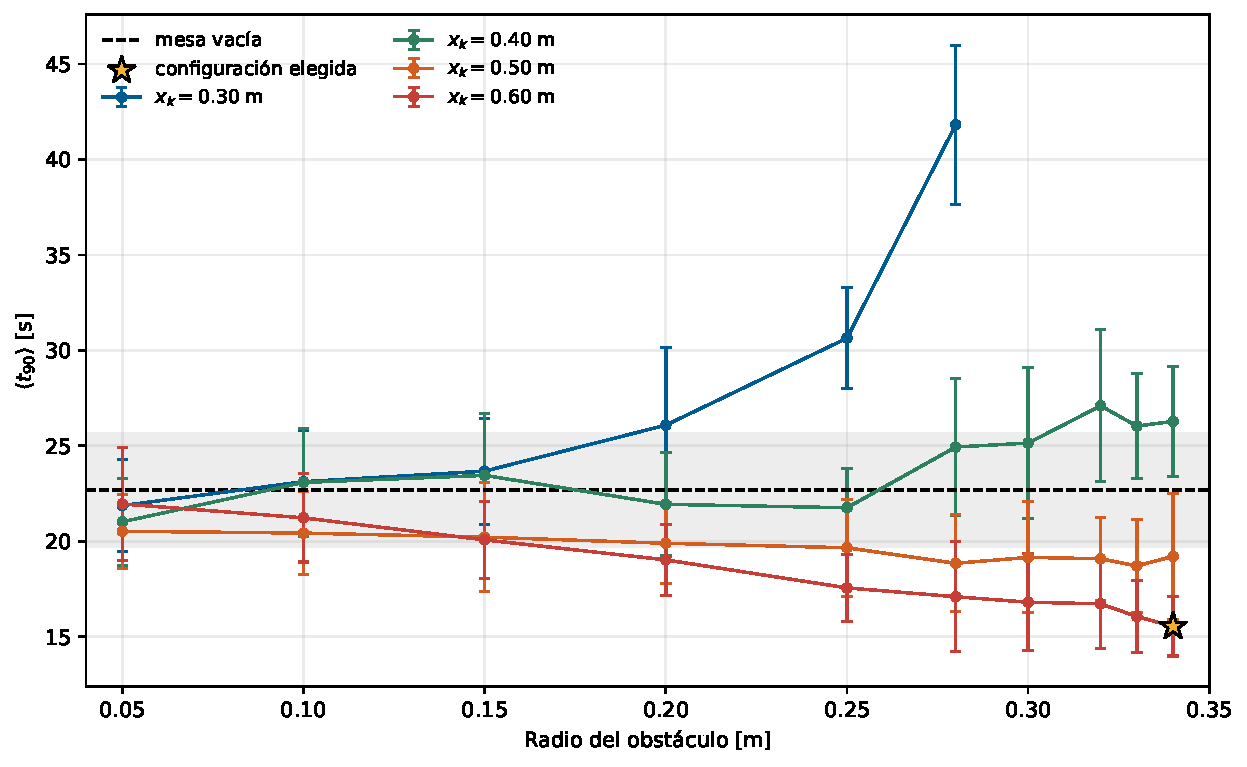
\includegraphics[width=\textwidth,height=5.1cm,keepaspectratio]{figuras/t90-vs-configuracion.pdf}
  \vspace{0.1em}
  \par\parametros{$N=100$; 15 realizaciones por punto; $t_{\max}=100\ \mathrm{s}$; variables: $x_k$ y $R_k$.\\
  Elegida: $K=1$, $(x_k,y_k,R_k)=(0{,}60;0{,}34;0{,}34)\ \mathrm{m}$; $\langle t_{90}\rangle=15{,}54\pm1{,}55\ \mathrm{s}$.}
\end{frame}

% 20
\begin{frame}{Coeficiente de difusión}
  \begin{columns}[T,onlytextwidth]
    \begin{column}{0.48\textwidth}
      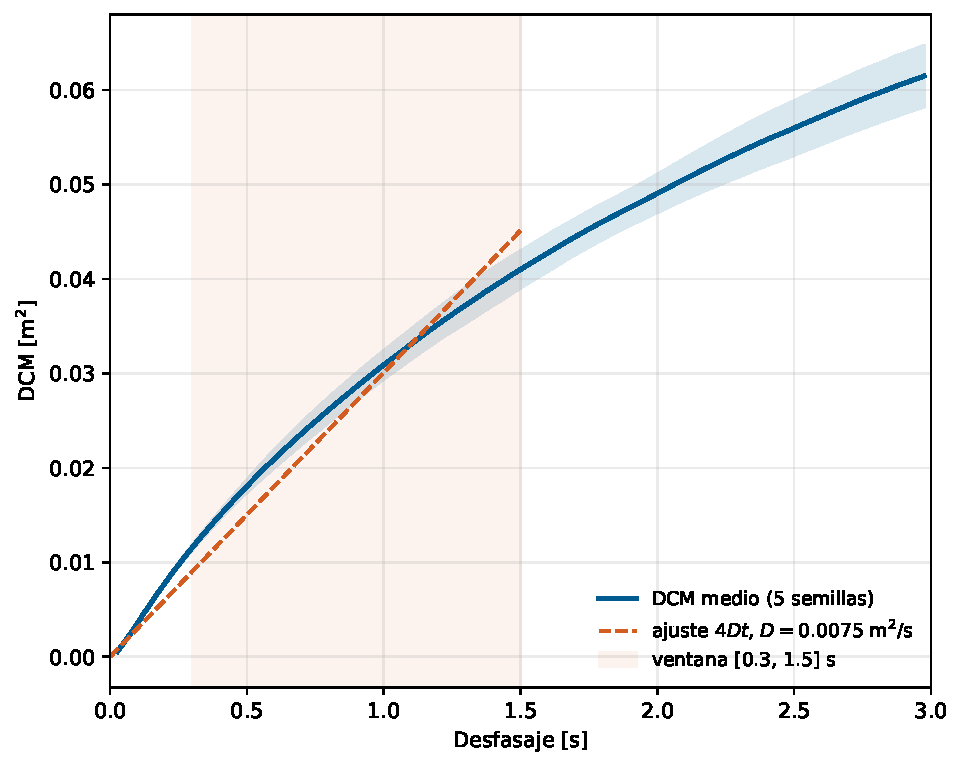
\includegraphics[width=\textwidth,height=5.0cm,keepaspectratio]{figuras/DCM-ajuste.pdf}
    \end{column}
    \begin{column}{0.48\textwidth}
      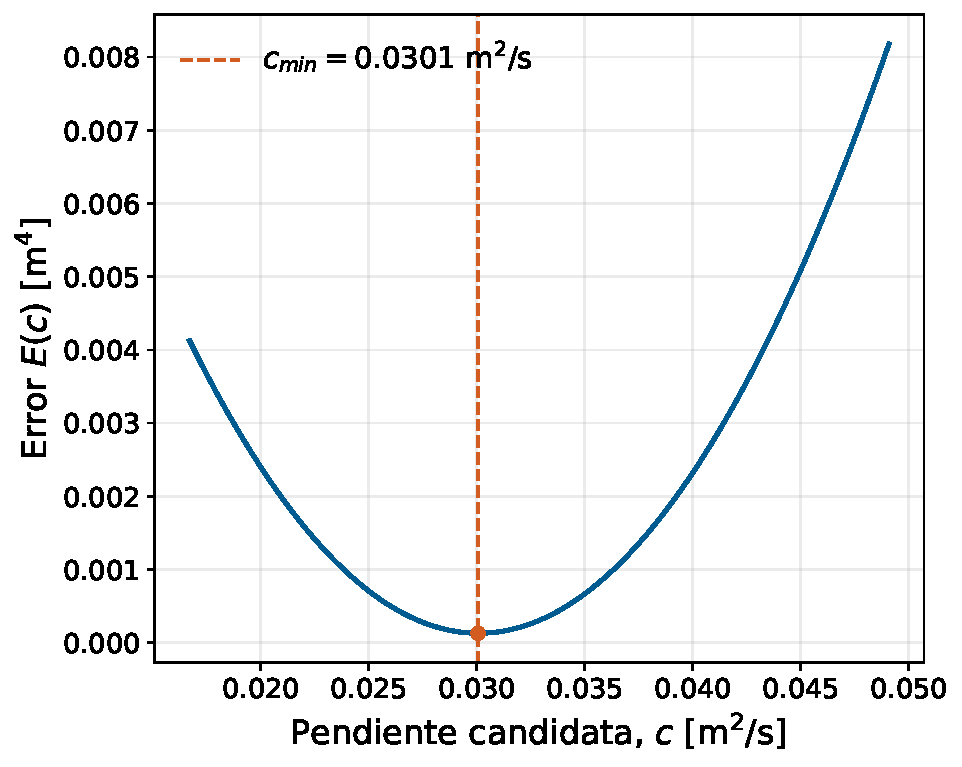
\includegraphics[width=\textwidth,height=5.0cm,keepaspectratio]{figuras/error-ajuste.pdf}
    \end{column}
  \end{columns}
  \vspace{0.15em}
  \centering\parametros{Configuración elegida; 5 semillas; ventana $[0{,}3;1{,}5]$ s; $\langle D\rangle=(0{,}00752\pm0{,}00036)\ \mathrm{m^2\,s^{-1}}$.}
\end{frame}

% 21
\begin{frame}{Difusión y tiempo al 90\,\%}
  \centering
  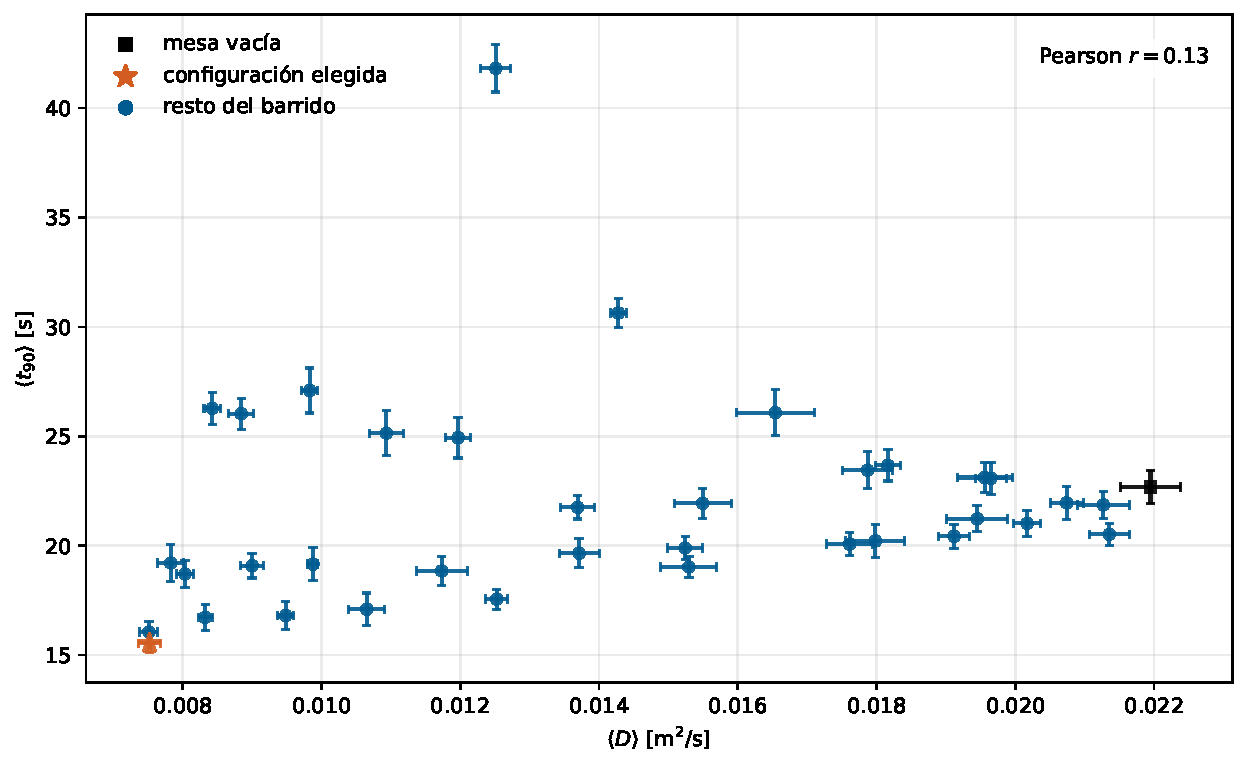
\includegraphics[width=\textwidth,height=5.25cm,keepaspectratio]{figuras/D-vs-t90.pdf}
  \vspace{0.2em}
  \par\parametros{$N=100$; 15 realizaciones para $t_{90}$ y 5 para $D$; barras: error estándar.\\
  En estas configuraciones, $D$ por sí solo no predijo $t_{90}$ ($r=0{,}13$).}
\end{frame}

% 22
\section{Conclusiones}
\begin{frame}
  \sectionpage
\end{frame}

% 23
\begin{frame}{Conclusiones}
  \begin{itemize}
    \item El tiempo de ejecución creció como $N^{3{,}30}$ en el rango $50\leq N\leq400$.
    \item El obstáculo central de radio máximo redujo $\langle t_{90}\rangle$ un 31,5\,\% y también redujo su dispersión frente a la mesa vacía.
    \item En el barrido completo, $D$ y $t_{90}$ mostraron una correlación débil ($r=0{,}13$).
  \end{itemize}
\end{frame}

% 24
\begin{frame}
  \centering
  \vfill
  {\usebeamercolor[fg]{structure}\usebeamerfont{title}Gracias por su atención}
  \vfill
\end{frame}

\end{document}
